\documentclass{article}
\usepackage[utf8]{inputenc}
\usepackage{geometry}
\usepackage{varwidth}
\usepackage{graphicx, subcaption}
\usepackage{amsmath}
\usepackage{enumitem}
\usepackage[toc, page]{appendix}
\usepackage{natbib}
\usepackage{titling}
\usepackage{hyperref}
\usepackage{comment}
\renewcommand\maketitlehooka{\null\mbox{}\vfill}
\renewcommand\maketitlehookd{\vfill\null}

\graphicspath{ {./pictures/} }
\geometry{
a4paper,
total={170mm,237mm},
left=20mm,
top=30mm,
}


\title{Assignment 2 \\  Discrete-event simulation - Multiple queues and multiple servers \\ \large Stochastic Simulation \\University of Amsterdam\\
\href{https://github.com/vdesgrange/Stochastic_simulation_project}{https://github.com/vdesgrange/Stochastic\_simulation\_project}}
\author{James Kingsbury (13437542), Viviane Desgrange (13337688) }
\date{1st December 2020}

\begin{document}

    \begin{titlingpage}
        \maketitle
    \end{titlingpage}


    \section*{Abstract}
    Queueing theory is the study of waiting lines or queues. Queueing theory can be useful when analysing a wide range of problems which involve some elements of queue lengths or waiting times. In this assignment, instead of focusing on a specific application such as a supermarket or an assembly line, we will consider queues in the most general, abstract sense. This means the results we derive can then be replicated in any application of these sets of ideas. In this assignment, we focus on one particular metric, the expected wait time of an agent in the queue. We investigate how different model formulations impact on the mean and the variance of this metric. Special attention will be paid to varying the number of servers, system load, different queue types and different service-time distributions. We succeed in replicating our theoretical results with statistical significance and demonstrating how different values of $\rho$ require different optimum customer numbers. Additionally, we show that job-first scheduling is advantageous in reducing the wait time when the system is under high load. We found that a deterministic service-time distribution can lead to lower median wait times and other convenient statistical properties of our estimate. Finally, we found that one component of the hyper-exponential distribution tends to dominate the other component in relation to its impact on the wait time.

    \section*{Introduction}
    Queuing theory as a research area has its origins in the work of Agner Erlang. Erlang was a Danish statistician and mathematician who spent part of his career creating models to describe the switchboard system of the Copenhagen Telephone Exchange company. Erlang wanted to understand how many switchboard circuits were required to maintain a reasonable standard of telephone service and how many telephone operators were required to manage a given volume of calls. (Erlang, 1920) is Erlang's principal work on waiting times, assuming constant hold times.

    (Adan and Resing, 2002) describes some of the key features which characterise a queuing model. The first feature concerns how agents enter our system, the arrival process of customers. Often we model these with exponentially distributed inter-arrival times. In our model, customers will arrive individually, but it is relatively common for batch-arrivals to be modelled. We can also model the behaviour of customers, for instance some customers might choose to leave the system if they haven't been served for a certain period of time. In certain implementations these customers may come back at a later time if a queue is too large when they arrive.

    The completion of jobs in our system can be modelled as as a service time distribution, independent of the arrival-time distribution. We usually assume that the service time values are independent and identically distributed. We assume that agents are processed one at a time by each server (if there are multiple). The number of servers is often denoted as c. There may be just one server processing jobs, or there could be multiple.

    The server can be configured to have different disciplines, the most common being first in - first out (FIFO). In FIFO ordering the first agent to arrive is first in the queue. We will also explore an alternative disciple: shortest job first. In this scheme, servers are aware of the 'size' or time required to complete jobs in the queue, then jobs are completed in order of size, regardless of the order in which they arrive. Shortest job first scheduling is a discipline within the broader 'prioritised' scheduling category.

    Proposed in (Kendall, 1953), Kendall notation is the standard notation used to define and classify a queuing system. The notation has 3 components - a/b/c. The first letter specifies the inter-arrival time distribution and the second is the service time distribution. The third letter specifies the number of servers in our system. We can also add additional letters to the notation if we want to specify non-standard features. For instance, we could add an extra component k, to denote a limit on the size of our queue or a component D to denote that we want to implement non-standard queuing discipline such as shortest job first scheduling. In the model implemented in our paper, customers arrive individually and there is no restriction on the queue size.

    For queuing systems with Poisson arrivals, we understand that the PASTA property holds (Willig, 1999). The PASTA acronym stands for poisson arrivals see time averages. This property states that the fraction of agents finding on arrival the system in some state A is the same as the fraction of time the system spend in state A. Note that deterministic queuing models do not have the PASTA property. Look at a D/D/1 system with arrivals at 1, 3, 5 and E(B) = 1. Each agent will arrive in the system finding it empty, however, it is only empty $\frac{1}{2}$ of the time.



    \newpage

    \section{Theory}

    \subsection*{Average waiting times and queuing theory}

    The queuing theory tells that $E(W)$ is smaller for a $M/M/c$ queue (with system load $\rho$, capacity $\mu$ and number of servers $c$) than for $M/M/1$ queue following the first in - first out discipline.
    As the main objective of our paper focus on the understanding of queue system for tasks management, we would like to verify this assumption. Therefore, we need to determine the average waiting time $E(W)$ with FIFO scheduling, to do so, we consider the general case $M/M/c$ using exponential distribution.\\
    \begin{itemize}
        \item First, we suppose that $\rho = \frac{\lambda}{c\mu}$, the fraction of time during which the $c$ servers are working, is smaller than 1 (to ensure that the queue length remains manageable).
        \item Second, we note $p_n$ the equilibrium probability to have $n$ jobs in the system, thus $\sum_{n=0}^{\inf} p_n = 1$
    \end{itemize}

    As we know the current state on the system depends on the number of jobs in the system, we can represent the system as a flow diagram (See Figure \ref{fig:flow_diagram_mmc}), where the node represents the  the different states of our system (number of jobs) and the arrows the transition from one state to the following:

    \begin{figure}[!ht]
        \centering
        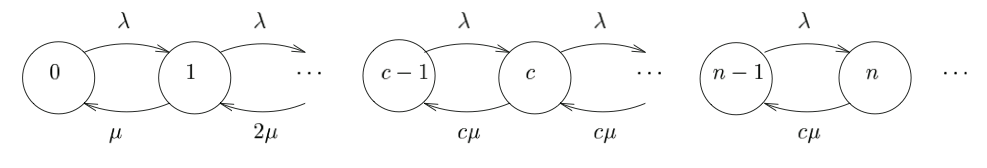
\includegraphics[width=.9\textwidth]{pictures/part_1/flow_diagram_mmc.png}
        \caption{Flow diagram for $M/M/c$ queue. (Adan, Resing, 2002.  Queueing Theory)}
        \label{fig:flow_diagram_mmc}
    \end{figure}

    A transition from a state $n$ to the state $n+1$ ($+1$ job) occur at the arrival rate $\lambda$.
    However, since we have $c$ servers, the transition from a state $n$ to a state $n-1$ occur at capacity (departure) rate $min(n, c) \mu$.

    Then, we can express $p_n$, the equilibrium probability to have n jobs in the system as:

    \begin{align}
        p_n = \frac{\lambda}{min(n, c) \mu} p_{n - 1}
    \end{align}

    If we iterate, we see that :
    \begin{equation}
        p_n = \Big(\frac{\lambda}{\mu} \Big)^n \Big(\frac{1}{min(n, c)} .  \frac{1}{min(n - 1, c)} \ldots \Big) p_0
    \end{equation}

    So, we consider 2 cases: a first case where the number of servers $c$ greater or equal to the number of jobs $n$; and a second case where the number of jobs $n$ is greater than $c$.\\
    So, if $n \leq c$, with $n = 0, \ldots, c$, then

    \begin{align}
        p_n &= \Big( \frac{\lambda}{\mu} \Big)^n \frac{1}{n!} p_0
        = \Big( \frac{\lambda}{\mu} \Big)^n \frac{c^n}{n! c^n} p_0
        = \Big( \frac{\lambda}{c \mu} \Big)^n \frac{c^n}{n!} p_0
        = \frac{(c \rho)^n}{n!} p_0\\
    \end{align}

    And if $c < n$, let's have $m = 0, 1, \ldots$ with $c + m \leq n$:

    \begin{align}
        p_{c + m} = \frac{1}{c! \underbrace{c \times c \times \ldots}_{\times m}} \Big( \frac{\lambda}{\mu} \Big)^{c + m} p_0
        = \frac{1}{c^m} \frac{1}{c!} \frac{c^c}{c^c} \Big( \frac{\lambda}{\mu} \Big)^c \Big( \frac{\lambda}{\mu} \Big)^m p_0
        = \frac{(c \rho)^c}{c!} \frac{1}{c^m} \Big( \frac{\lambda}{\mu} \Big)^m p_0
        = p_c \rho^m
        \label{eq:p_c_plus_m}
    \end{align}

    We now have a new mathematical definition of the equilibrium probability $p_n$.
    But in order to determine $E(W)$, we must also determine the case $p_0$, required for the last part of the demonstration.\\
    As we know that the equilibrium probabilities are such that $\sum_{n=0}^{\inf} p_n = 1$, therefore we have:

    \begin{align}
        1 &= \lim_{N\to\infty} \sum_{n=0}^{c - 1} p_n + \sum_{m=0}^{N} p_{c + m} \\
        1 &= \lim_{N\to\infty} \sum_{n=0}^{c - 1} \frac{(c \rho)^n}{n!} p_0 + \sum_{m=0}^{N} \rho^m \frac{(c \rho)^c}{c !} p_0  \\
        p_0 &= \lim_{N\to\infty} \Big( \sum_{n=0}^{c - 1} \frac{(c \rho)^n}{n!} + \frac{(c \rho)^c}{c !} \sum_{m=0}^{N} \rho^m \Big)^{-1}
    \end{align}

    To simplify our result, we should remember that :

    \begin{align}
        \sum_{m=0}^{N} \rho^m &= 1 + \rho + \rho^2 + \ldots + \rho^N = \frac{\rho^{N + 1} - 1}{\rho - 1} \\
        \lim_{N\to\infty} \sum_{m=0}^{N} \rho^m &= \frac{0 - 1}{\rho - 1} = \frac{1}{1 - \rho}
    \end{align}

    So we can define $p_0$ as:
    \begin{align}
        p_0 &= \lim_{N\to\infty} \Big( \sum_{n=0}^{c - 1} \frac{(c \rho)^n}{n!} + \frac{(c \rho)^c}{c !} \frac{1}{1 - \rho} \Big)^{-1}
        \label{eq:p0}
    \end{align}

    Given that our queuing system is defined with Poisson arrival (M/./.), we can use the PASTA property, and the Equation \ref{eq:p_c_plus_m}, to define the probability $\Pi_W$ that a job has to wait :

    \begin{align}
        \Pi_W &= p_c + p_{c+1} + p_{c+2} + \ldots \\
        \lim_{N\to\infty} \Pi_W &= \sum_{n=0}^{N} p_{c + n} = p_c \sum_{n=0}^{N} \rho^n = \frac{p_c}{1 - \rho}
        \label{eq:pi_w}
    \end{align}

    As we know from Equation \ref{eq:p0} that $p_c = \rho^0 \frac{(c \rho)^c}{c!}p_0$, we can transform the Equation \ref{eq:pi_w} :

    \begin{equation}
        \lim_{N\to\infty} \Pi_W = \frac{(c \rho)^c}{c !} \Big((1 - \rho) \sum_{n = 0}^{c-1}\frac{(c \rho)^n}{n !} + \frac{(c \rho)^c}{c !} \Big)^{-1}
    \end{equation}

    Let's now consider \emph{Little's Law}, which define the relation: $E(W) = E(L^q) \lambda^{-1}$, where $E(L^q)$ is the average length of the queue.
    $E(L^q)$ can be define as the summation of all the expected number of jobs $n$ beyond the capacity $c$ of the queue system. So we have (using Equation \ref{eq:pi_w}) :

    \begin{align}
        E(L^q) &= \sum_{n=0}^{\infty} n p_{c + n} = \sum_{n=0}^{\infty} n p_c \rho^n = \frac{p_c}{1 - \rho} \sum_{n=0}^{\infty} n (1 - \rho) \rho^n
        \label{eq:e_l_q}
    \end{align}

    And considering that:
    \begin{align}
        \sum_{n=0}^{\infty} n (1 - \rho) \rho^n &= 0 + (\rho - \rho^2) + (2\rho^2 -2\rho^3) \ldots = 0 + \rho + \rho^2 + \rho^3 + \ldots \\
        \sum_{n=0}^{\infty} n (1 - \rho) \rho^n &= \lim_{N\to\infty} \frac{\rho^{N + 1} - 1}{\rho - 1} - 1 = \lim_{N\to\infty} \frac{\rho}{1 - \rho}
    \end{align}

    Then we can transform the Equation \ref{eq:e_l_q}:

    \begin{align}
        E(L^q) &= \lim_{N\to\infty} \Pi_W \sum_{n=0}^{N} n (1 - \rho) \rho^n = \Pi_W \frac{\rho}{1 - \rho}
        \label{eq:e_l_q}
    \end{align}

    Finally, from the \emph{Little's Law} relation $E(W) = E(L^q) \lambda^{-1}$, from the Equation \ref{eq:pi_w}, the Equation \ref{eq:e_l_q} and the relation $\rho = \frac{\lambda}{c\mu}$;we obtain the definition of $E_c(W)$ for an $M/M/c$ queue:

    \begin{equation}
        E_c(W) = \frac{(c \rho)^c}{c !} \Big((1 - \rho) \sum_{n = 0}^{c-1}\frac{(c \rho)^n}{n !} + \frac{(c \rho)^c}{c !} \Big)^{-1} \frac{1}{1 - \rho} \frac{1}{c \mu}
    \end{equation}

    From which, we can derive the average waiting time for an $M/M/1$ queue:
    \begin{equation}
        E_1(W) =  \frac{\rho}{(1 - \rho)\mu}
    \end{equation}

    Now that we know the average waiting time equation for $M/M/c$ queues, we can compute the theoretical values for variation of parameters $\rho$ and $c$ (See Tables \ref{Table:ew_by_number_servers_theoretical_results} and \ref{Table:ew_by_rho_single_server_theoretical_results}).
    As suggested by queuing theory, it appears that for FIFO scheduling a greater number of servers $c$ in a $M/M/c$ queue will results in shorter average waiting times, for same system load $\rho$ and processor capacity $\mu$.
    In the next part of the paper we will test these theoretical results again the estimated $E_c(W)$ values obtained from our simulation.

    \begin{table}[h!]
        \parbox{.48\linewidth}{
        \centering
        \begin{tabular}{|c | c |}
            \hline
            $c$ & $E_c(W)$ \\
            \hline\hline
            1 & 9.000 \\
            2 & 4.263 \\
            3 & 2.723\\
            4 & 1.969 \\
            \hline
        \end{tabular}
        \caption{$E_c(w)$ with $\rho = 0.9$ and $\mu = 1$}
        \label{Table:ew_by_number_servers_theoretical_results}
        }
        \parbox{.48\linewidth}{
        \centering
        \begin{tabular}{|c | c || c | c |}
            \hline
            $\rho$ & $E_1(W)$ & $\rho$ & $E_1(W)$ \\
            \hline\hline
            0.10 & 0.11 & 0.60 & 1.50\\
            0.20 & 0.25 & 0.70 & 2.33 \\
            0.30 & 0.43 & 0.80 & 4.00 \\
            0.40 & 0.67 & 0.90 & 9.00 \\
            0.50 & 1.00 & 0.95 & 19.0 \\
            \hline
        \end{tabular}
        \caption{$E_1(w)$ $\mu = 1$}
        \label{Table:ew_by_rho_single_server_theoretical_results}
        }
    \end{table}

    \newpage

    \section{Results}
    \subsection*{Verifying Theoretical Wait Time Results}

    Now that we have derived the theoretical E(w) times, we will simulate our queuing system and estimate the expected wait times. In our first experiment, we will simulate our queuing system 50 times, with each simulation having 5000 total customers. After each simulation we obtain the mean wait time and form a sample of mean wait times to perform statistics on. We will obtain estimates of $E_1(W), E_2(W)$ and $E_4(W)$ given $\rho = 0.9$. In our previous assignment, (Desgrange \& Kingsbury, 2020), sample variance and t test methods were explained and derived which we will use again here.

    \begin{table}[h!]
        \parbox{.48\linewidth}{
        \centering
        \begin{tabular}{|c | c | c | c|}
            \hline
            C & $E_c(W)$ & Sample Variance \\
            \hline\hline
            1 & 8.987 & 3.027 \\
            2 & 4.028 & 0.636 \\
            4 & 1.888 & 0.150 \\
            \hline
        \end{tabular}
        \caption{}
        \label{Table:ew_sim_results}
        }
        \parbox{.48\linewidth}{
        \centering
        \begin{tabular}{|c | c | c | c|}
            \hline
            C & Test Statistic & P-Value \\
            \hline\hline
            1 & -0.984 & 0.329 \\
            2 & -1.665 & 0.102 \\
            4 & -1.397 & 0.168 \\
            \hline
        \end{tabular}
        \caption{}
        \label{Table:ttest_results}
        }
    \end{table}

    Table~\ref{Table:ew_sim_results} shows the results obtained from our initial simulations. Intuitively, as the number of available counter slots increases, the $E_c(W)$ also decreases. To test whether the $E_c(W)$ results obtained from our simulation are considered to be equal with statistical significance to those derived theoretically, we will run 3 t-tests on our 3 obtained mean values. Our null hypothesis is that $E_c(W) = X_c$ where $X_c$ represents the theoretical wait time in a queue with $c$ servers and $E_c(W)$ is our simulated wait time.

    The critical values for the test statistics in Table~\ref{Table:ttest_results} can be obtained through $T_{n-1}^{-1}(\frac{p + 1}{2})$. If the absolute value of our test statistic is lower than the critical value then we fail to reject the null hypothesis that the mean of our $E_c(W)$ value is equal to some value $\mu$, which in our case is the theoretical result for wait time. The p-values in Table~\ref{Table:ttest_results} can be interpreted as the probability that we observe results as extreme as our sample, given that the null hypothesis of our test is correct. Very small p-values suggest that the obtained result is very unlikely if the null hypothesis is correct. Since our p-values are larger than $\alpha = 0.05$, we fail to reject the null hypothesis, our experimental results do not appear to deviate significantly from the theoretical results obtained.\\

    \begin{figure}[!ht]
        \centering
        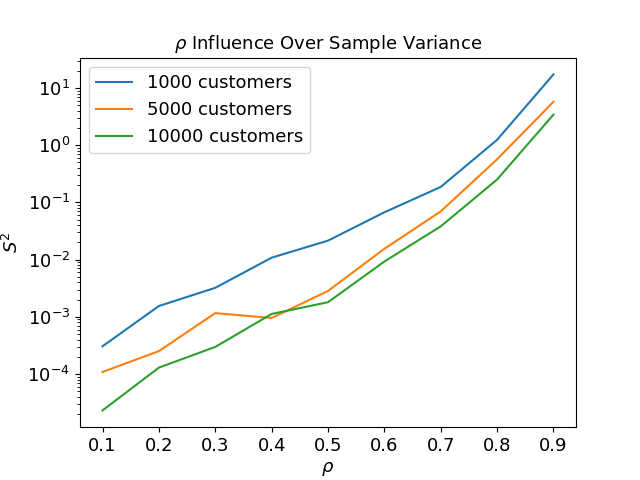
\includegraphics[width=0.75\textwidth]{pictures/part_2/samp_var_q2.png}
        \caption{Given $\mu = 1$ and $\lambda = 1$, see how the sampling variance of our estimate varies.  }
        \label{fig:samp_var}
    \end{figure}

    \subsection*{Influence of system load $\rho$ over average waiting time $E_c(W)$}

    All of the experiments above were conducted with a relatively high value of $\rho$ and a large number of customers and repeat simulations. However, we are interested in how the estimate of the sample mean of $E_c(W)$ varies as we vary the value of $\rho$. Do we observe a higher variance of our sample mean estimator as we increase the value of $\rho$? Figure~\ref{fig:samp_var} shows the results of an experiment which aims to investigate how the sample variance of our mean waiting time evolves as we increase $\rho$. The experiment was run with parameters $\mu = 1$, $c = 1$ and the sample variance of our $E_1(W)$ estimate over 30 simulation runs is measured on the y axis. Sample variance increases superlinearly with $\rho$, note the log scale on the Y-axis. As the system load increases, wait times become more unpredictable for any given agent joining the queue. In an overloaded system, one abnormally long sampled service time has a large effect on the wait time of all agents in the queue, leading to more unpredictable wait times on average. We note that for any given level of $\rho$, the variance of our estimator tends to be reduced the greater the number of total customers.\\

    \begin{figure}[!ht]
        \centering
        \begin{subfigure}{.47\textwidth}
            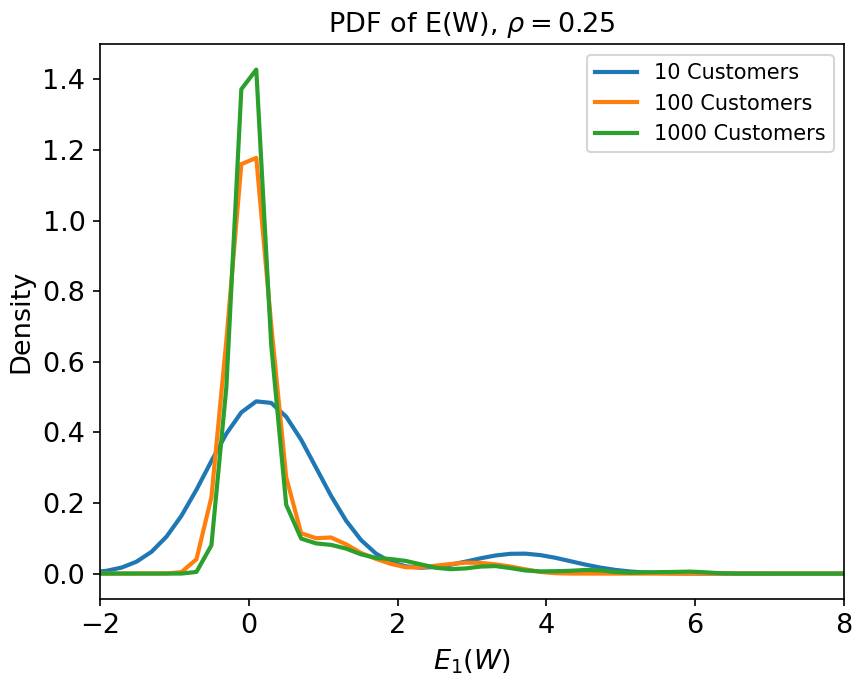
\includegraphics[width=\textwidth]{pictures/part_2/pdf,025.png}
            \caption{Probability density function for varying numbers of total customers, $\rho = 0.25$, $c = 1$}
            \label{fig:pdf_1}
        \end{subfigure}
        \begin{subfigure}{.47\textwidth}
            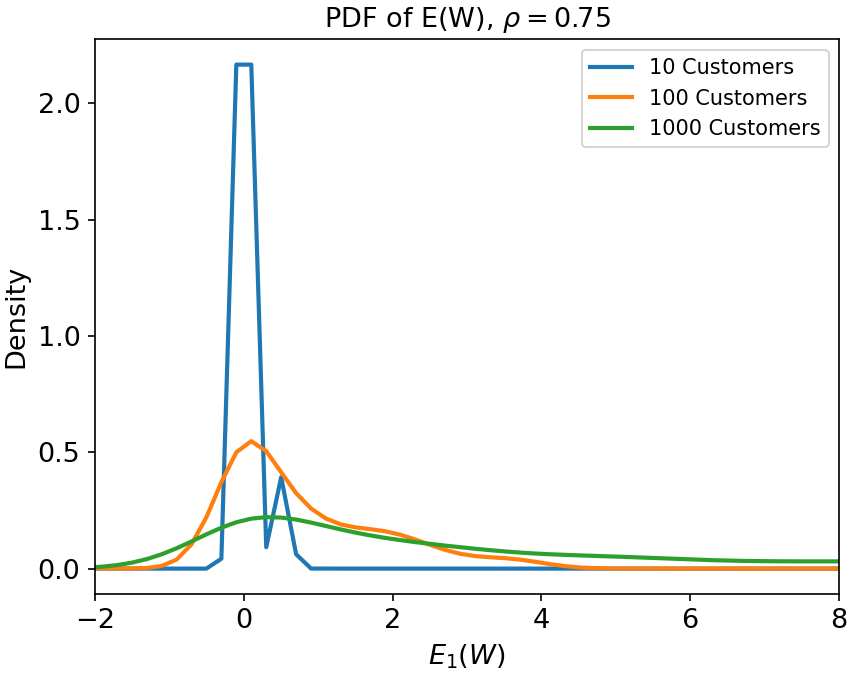
\includegraphics[width=\textwidth]{pictures/part_2/pdf,075.png}
            \caption{Probability density function for varying numbers of total customers, $\rho = 0.75$, $c = 1$}
            \label{fig:pdf_2}
        \end{subfigure}
    \end{figure}

    We now want to investigate how the number of measurements required to attain statistical significance depends on $\rho$. Ideally, the distribution of our mean expected wait times should approximate a normal distribution, so that we can reliably investigate the statistical properties of our estimates.\\
    Figure~\ref{fig:pdf_1} and Figure~\ref{fig:pdf_2} shows how the probability density function of our $E_1(W)$ estimate changes as we vary the total number of customers in our system. For a lower value of $\rho$, we obtain a more normal like distribution if we use a higher number of total customers. We obtain a more asymmetric long-tail distribution if we use a lower number of total customers. For a higher value of $\rho$, the inverse is true. We obtain a more normal-like density function if we use a lower number of total customers and a more distorted distribution if we use a higher number of total customers. We suggest this to be because when our system is overloaded, a large value sampled from the service time distribution can cause a 'ripple' effect on the wait time of all agents currently in the queue. So only processing 10 total customers means there is less chance of sampling one of these extreme values from the long-tail of the exponential distribution and thus our expected mean is more likely to approximate a normal distribution. Whereas, for lower values of $\rho$, one extreme service time has little effect on other agents in the system.\\

    \subsection*{Influence of jobs scheduling system : FIFO and Priority queue}

    The next step consists in investigating how the job scheduling system influence on the efficiency of average waiting time.
    Indeed, in a first time we focused our attention on the first in - first out (FIFO) scheduling which did not consider job size, while this parameter can logically influence the rapidity of processing, and so the average waiting time.
    Therefore, we studied the non-preemptive priority queue system, which gives greater priority to smallest job in scheduling, without allowing interruption of smaller priority jobs by greater priority jobs.\\

    As our experiments were done with \emph{Simpy} framework, we decided of the usage of \emph{PriorityResource} object which accept a priority \emph{integer} parameter associated to each jobs.
    Here, we must emphases the existence of an error we tried to minimize: as our job service time is determined by exponential distribution, it is a \emph{float} variable. To provide this \emph{float} directly to \emph{PriorityResource} object would results in a conversion with a lost of precision, and an error in job scheduling.\\
    We considered 2 solutions:
    \begin{enumerate}
        \item A simple function which return an int from a float while keeping some precision: $f(x) = x * 10^8$. However, it only minimize the error, it remains an approximation of real job ordering.
        \item Use the geometric distribution, discrete version of exponential distribution.
    \end{enumerate}
    For the sake of convenience, we decided to start our experiments with the simple conversion.\\

    In this experiment we run 50 simulations with a total of 10,000 jobs. We store the average waiting time from each simulation then study its distribution. We fix the servers capacity $\mu = 1$ in a first time, and observe for different values of $\rho$. We will next observe the evolution of sample variance $S^2$ and sample mean $E_c(W)$ by $\rho$ in a second time.
    Our assumption is that job scheduling by priority should improve the average waiting time $E_c(W)$ but also influence the variance given that waiting time will be influence by priority while it was only influence by exponential distribution of the jobs in the FIFO system.

    \begin{figure}[h]
        \centering
        \begin{subfigure}[b]{0.47\textwidth}
            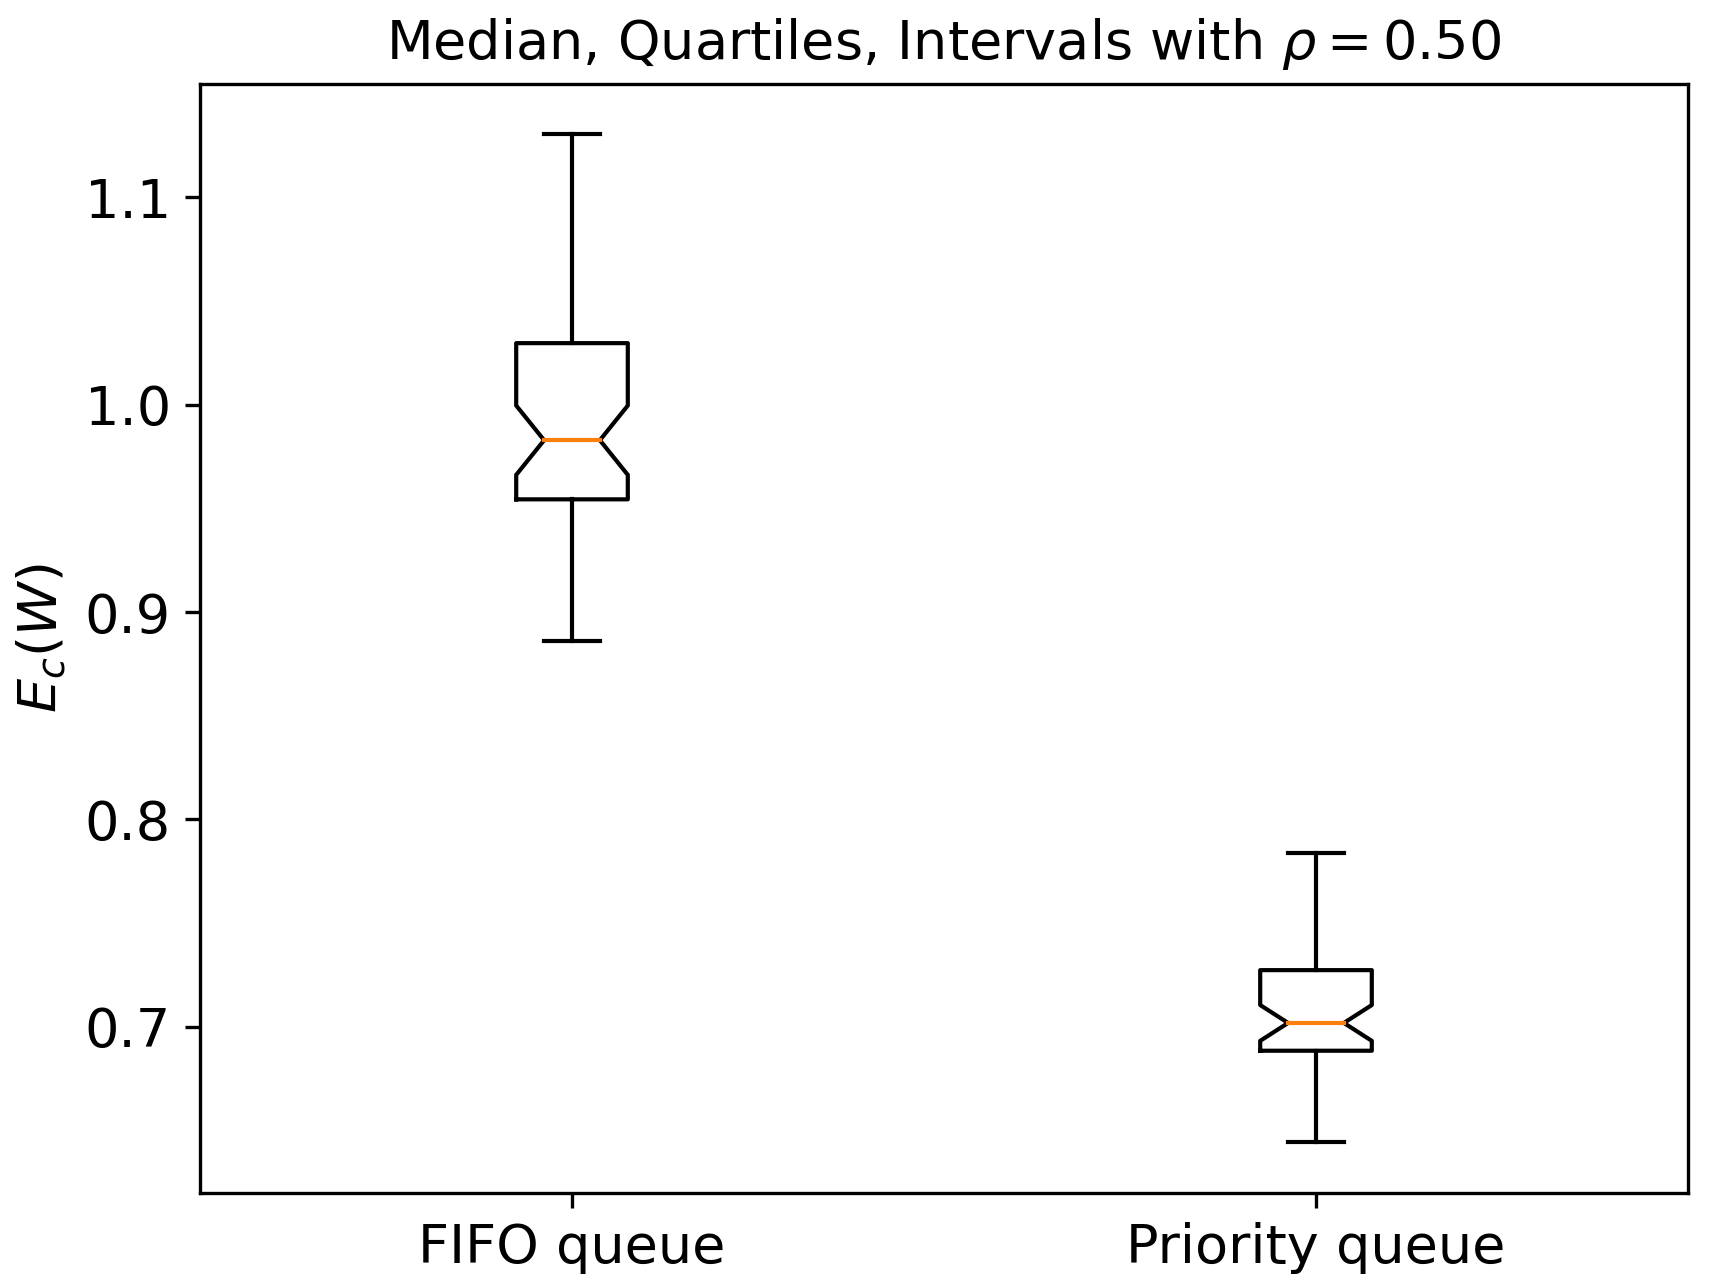
\includegraphics[width=\textwidth]{pictures/part_3/box_plot_rho_050.png}
            \caption{Notched Box Plot, $\rho = 0.5$}
            \label{fig:q3_notchedbox_050}
        \end{subfigure}
        \begin{subfigure}[b]{0.47\textwidth}
            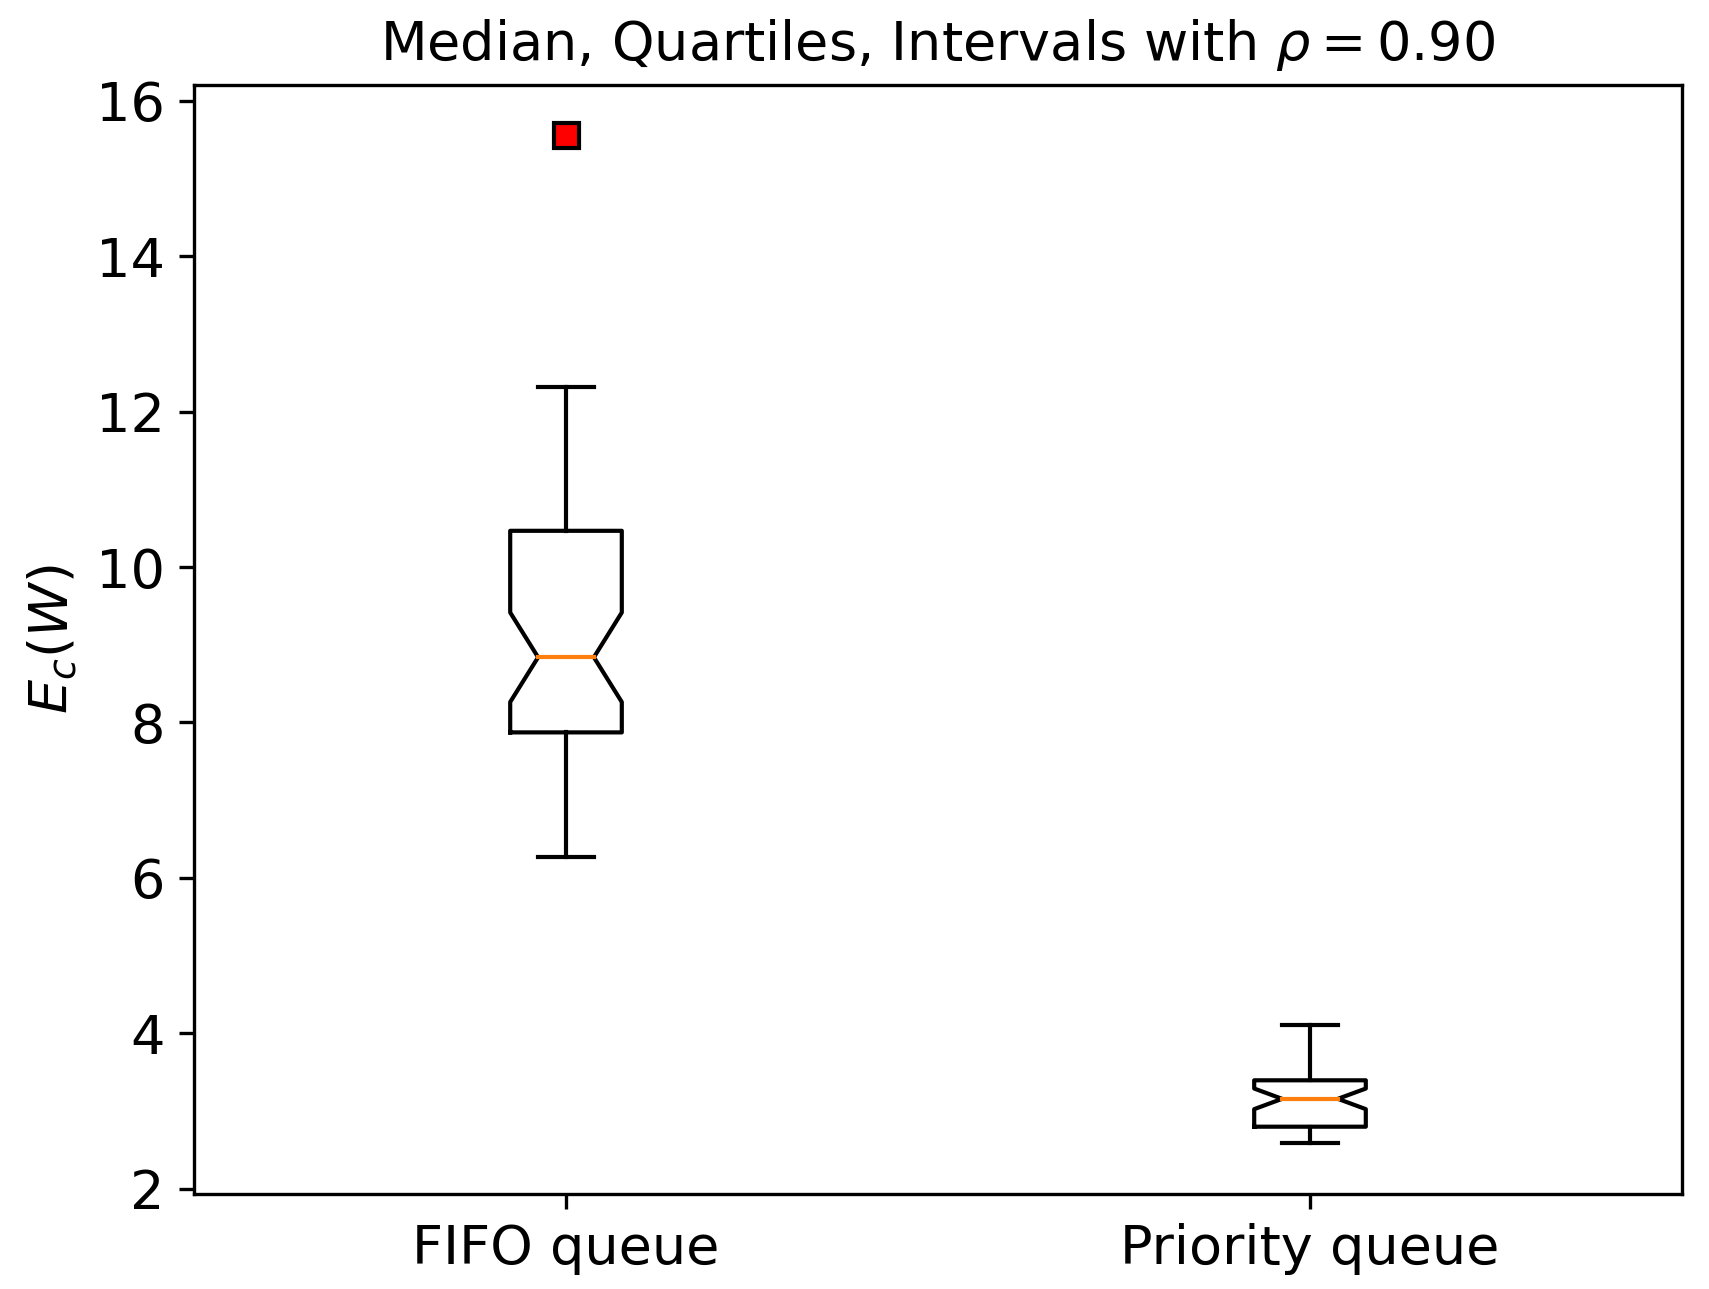
\includegraphics[width=\textwidth]{pictures/part_3/box_plot_rho_090.png}
            \caption{Notched Box Plot, $\rho = 0.9$}
            \label{fig:q3_notchedbox_090}
        \end{subfigure}
        \caption{$E_c(W)$ distribution in FIFO and Priority queues}
        \label{fig:fifo_vs_priority}
    \end{figure}

    \begin{figure}[h]
        \begin{subfigure}[b]{0.48\textwidth}
            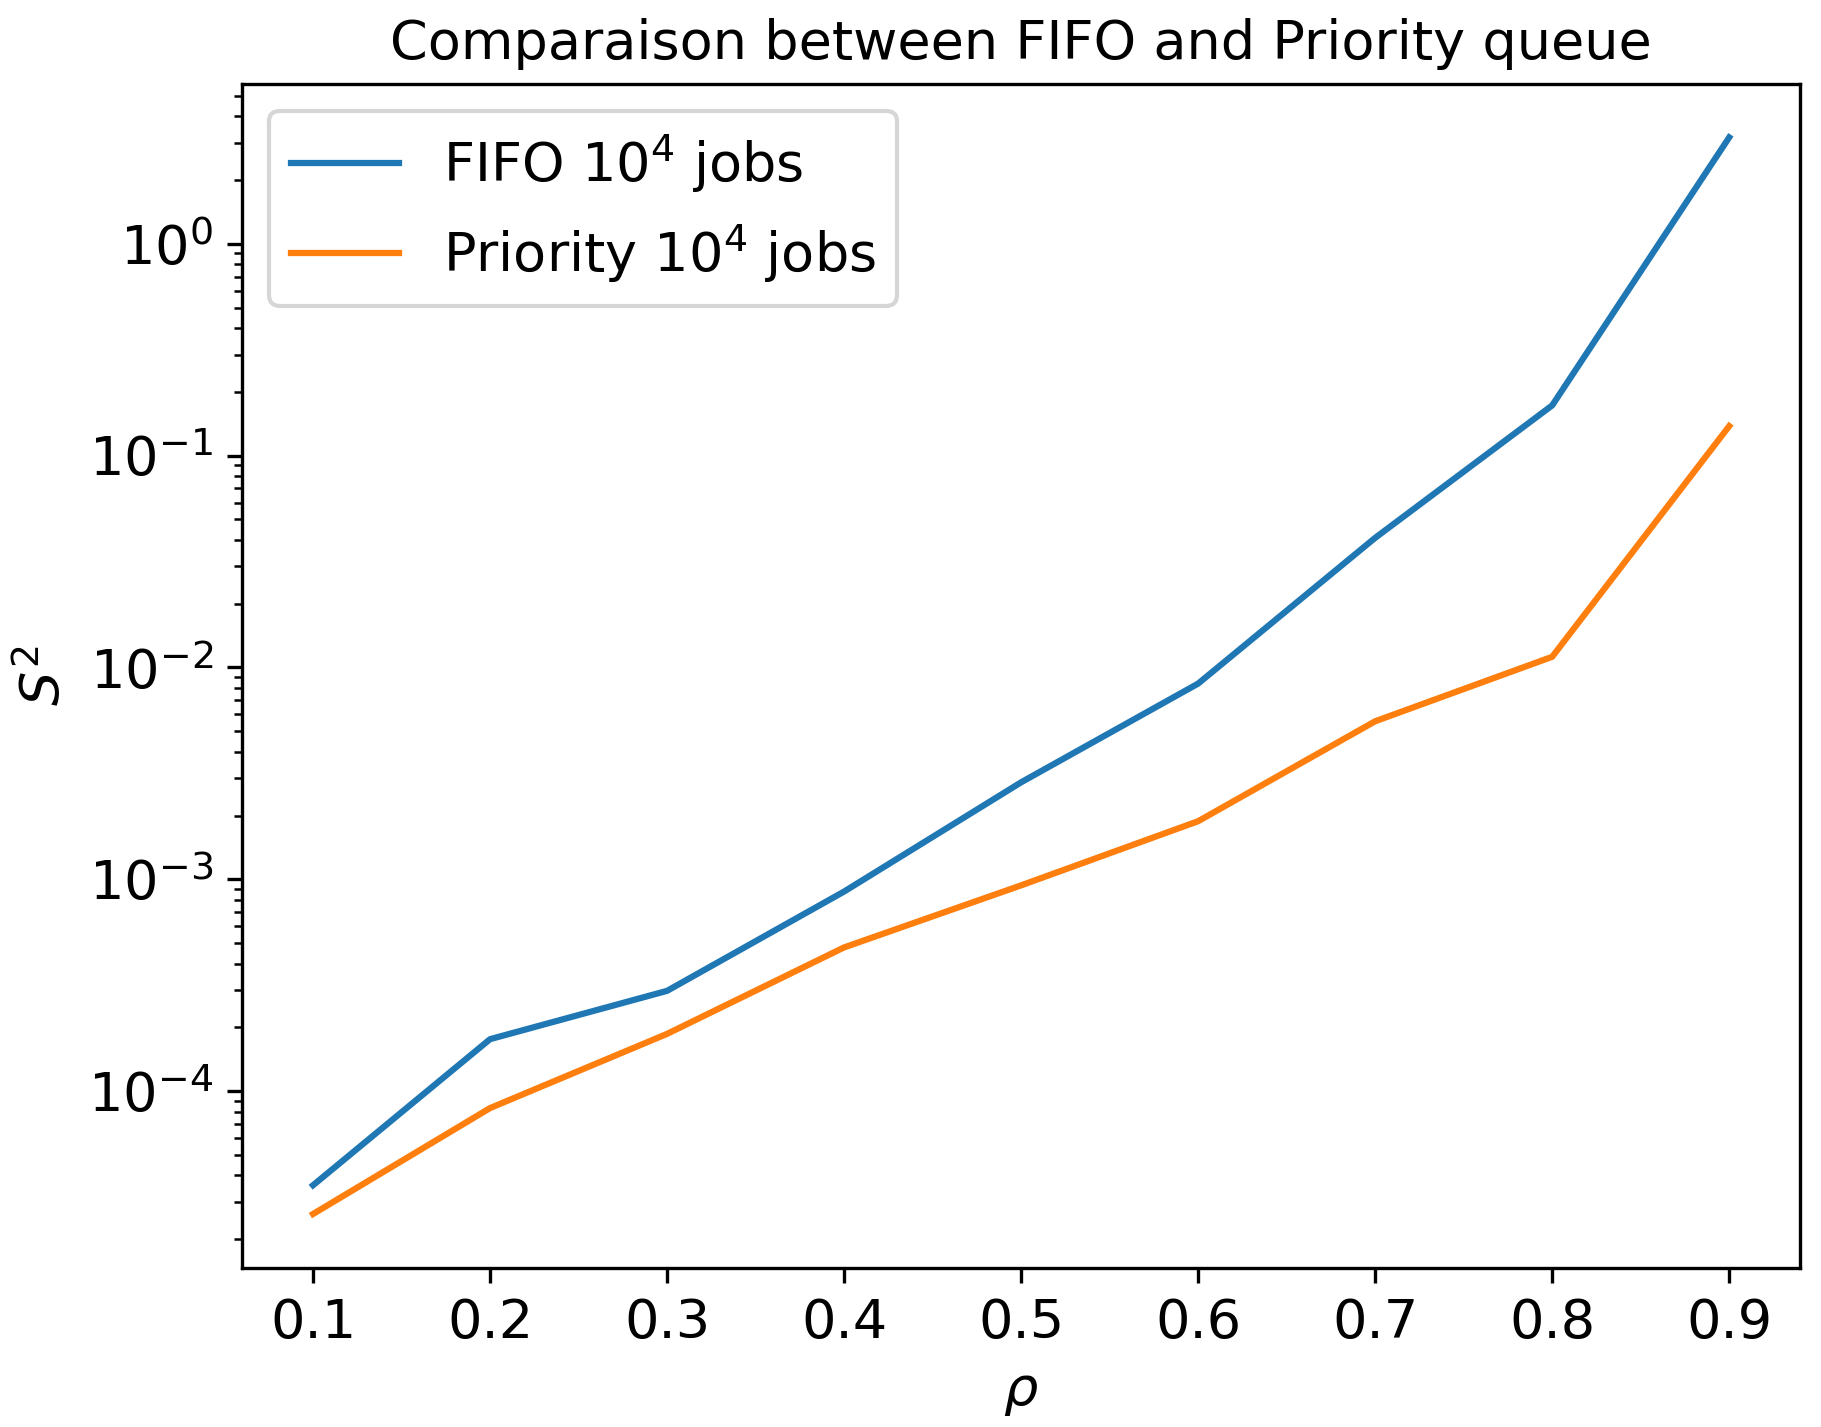
\includegraphics[width=\textwidth]{pictures/part_3/sample_variance_fifo_priority.png}
            \caption{Sample Variance Comparison, Semi-log Plot}
            \label{fig:q3_samp_var}
        \end{subfigure}
        \begin{subfigure}[b]{0.45\textwidth}
            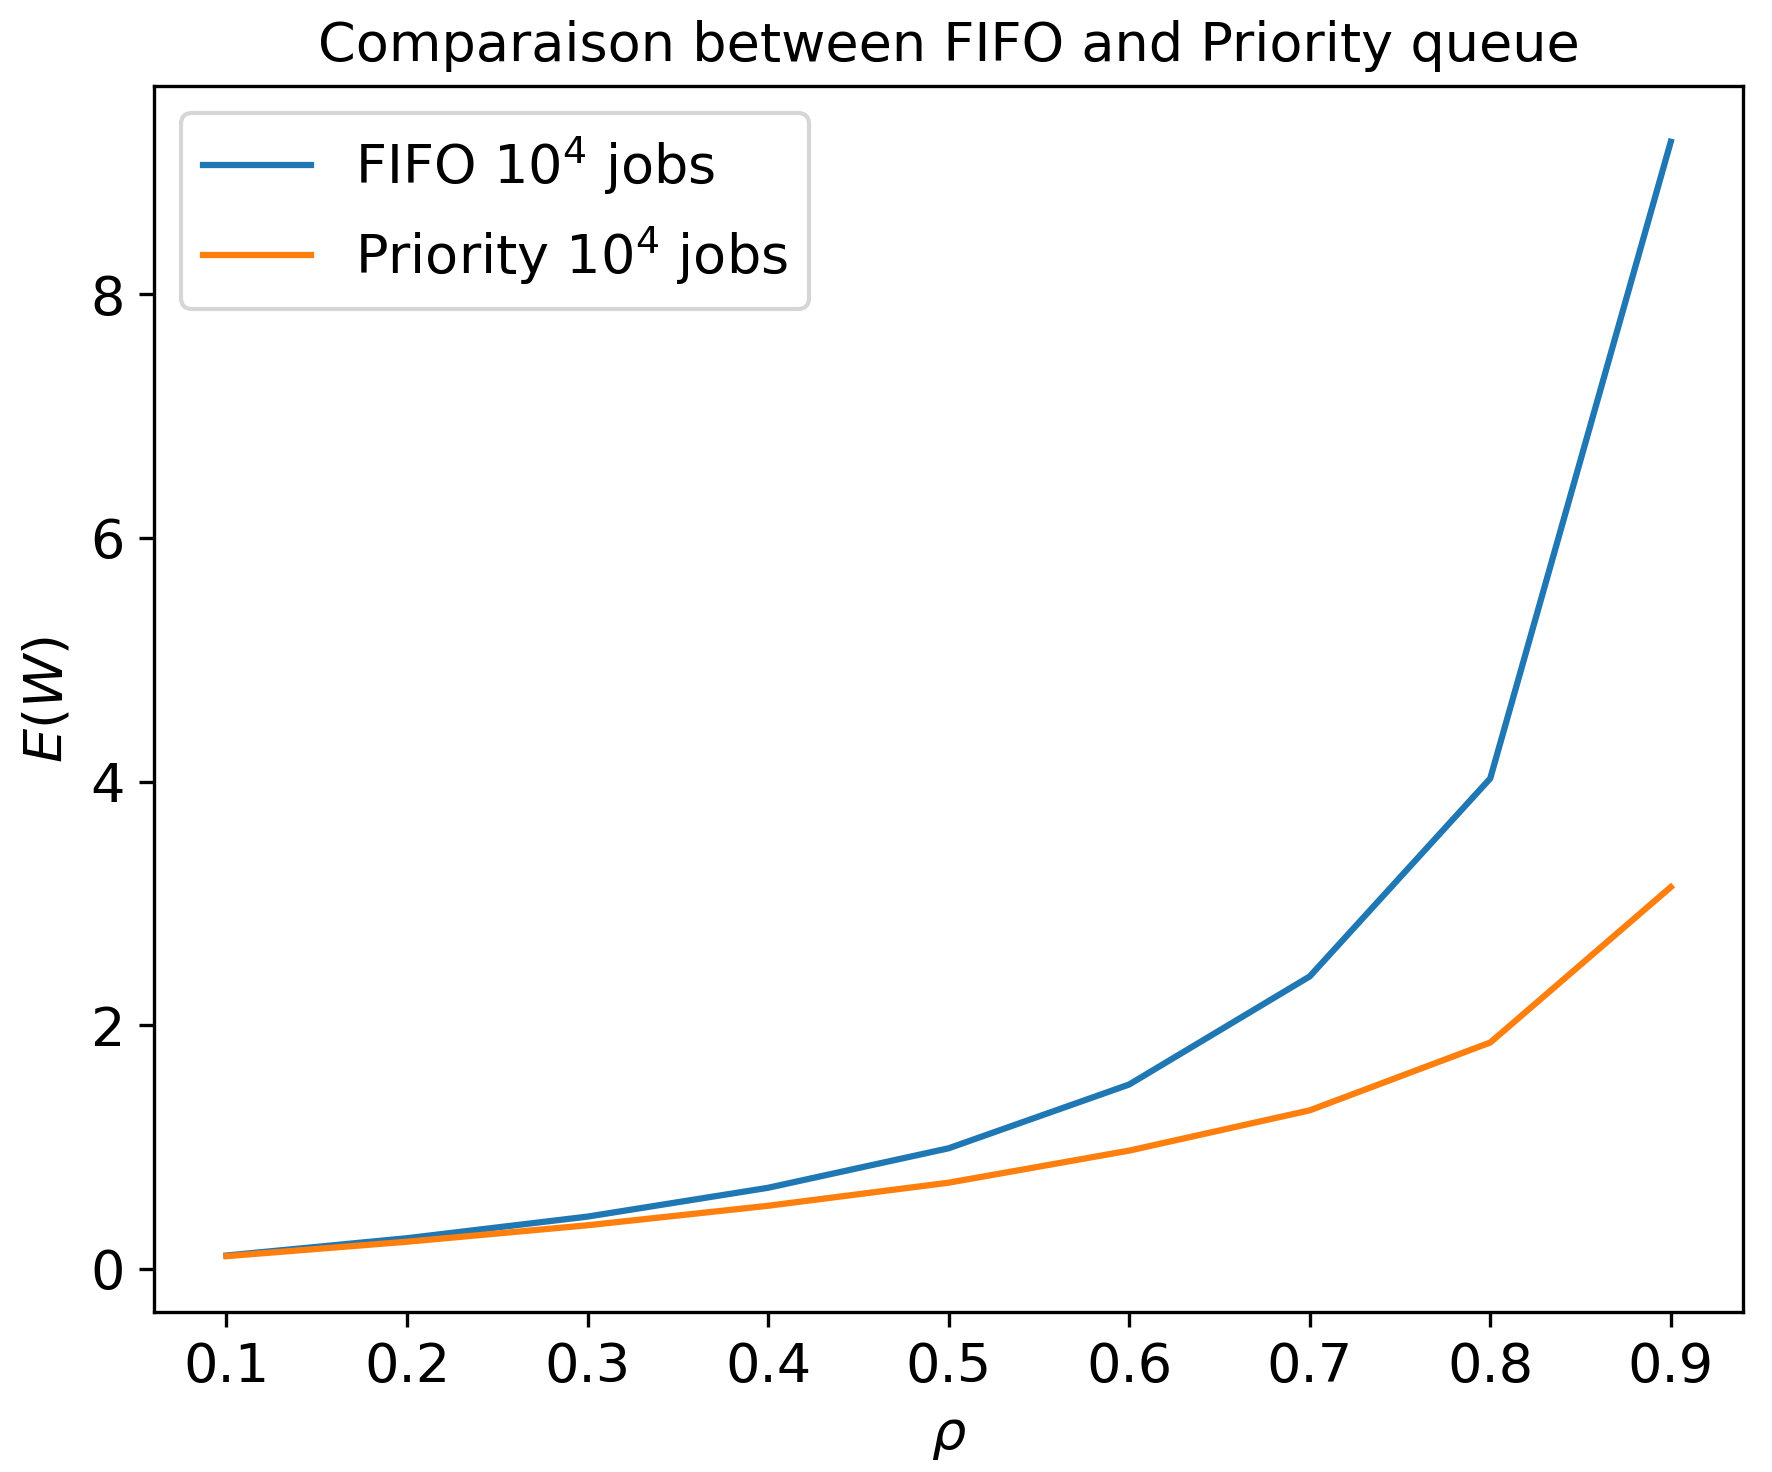
\includegraphics[width=\textwidth]{pictures/part_3/sample_mean_fifo_priority.png}
            \caption{Sample mean Comparison}
            \label{fig:q3_samp_mean}
        \end{subfigure}
        \caption{FIFO vs Priority queue}
        \label{fig:fifo_vs_priority_samp_mean_var}
    \end{figure}

    The Figure \ref{fig:q3_notchedbox_050} and \ref{fig:q3_notchedbox_090} make use of notched box plots to describe the distribution of $E_c(W)$ (with $c = 1$) for $\rho = 0.5$ and $\rho = 0.9$. The orange line for each parameter setting shows the median $E_c(W)$ value. The box extends to the upper and lower quartiles of the median value. The notch in the side of each of the boxes represents the 95\% confidence interval for this median, then the whiskers on the top and bottom of each box extend to the upper and lower limits of values. The outliers are represented as red points beyond the upper and lower limits. We observe a manifest improvement between FIFO scheduling $E_c(W)$ and shortest job-first scheduling as expected. The priority queue has a tighter confidence interval, lower median and smaller range than the equivalent FIFO queue for both $\rho = 0.5$ and $\rho = 0.9$.

    Additionally, the Figure \ref{fig:q3_samp_var} and \ref{fig:q3_samp_mean} which respectively shows evolution of sample variance $S^2$ and sample mean $E_1(W)$ confirms our first assumption: while the sample variance still depends on $\rho$ it is influenced by the priority job scheduling and at the same time, the average waiting time $E_1(W)$ is greatly improved.

    \subsection*{Influence of service rate distribution}

    We will now investigate how adopting a deterministic service time distribution affects the properties of our $E_c(W)$ estimate. We will run an experiment to compare the distribution of the mean waiting times obtained from an exponential service time distribution and those from a deterministic distribution. We run 50 simulations each having 10,000 total customers. We take the mean wait time in each simulation and create a distribution of mean wait times to perform statistical testing on. We use the parameters $\mu = 1$ and $\rho = 0.9$. Despite having shown in the previous section that an increased value of $\rho$ increases the sample variance, we still choose to use a high value of $\rho$ as the results in the this section are slightly clearer at this level. We hypothesize that the wait times under the deterministic scenario will have a lower average value and tighter confidence intervals owing to reduced sample variance.

    \begin{figure}[h]
        \centering
        \begin{minipage}[b]{0.45\textwidth}
            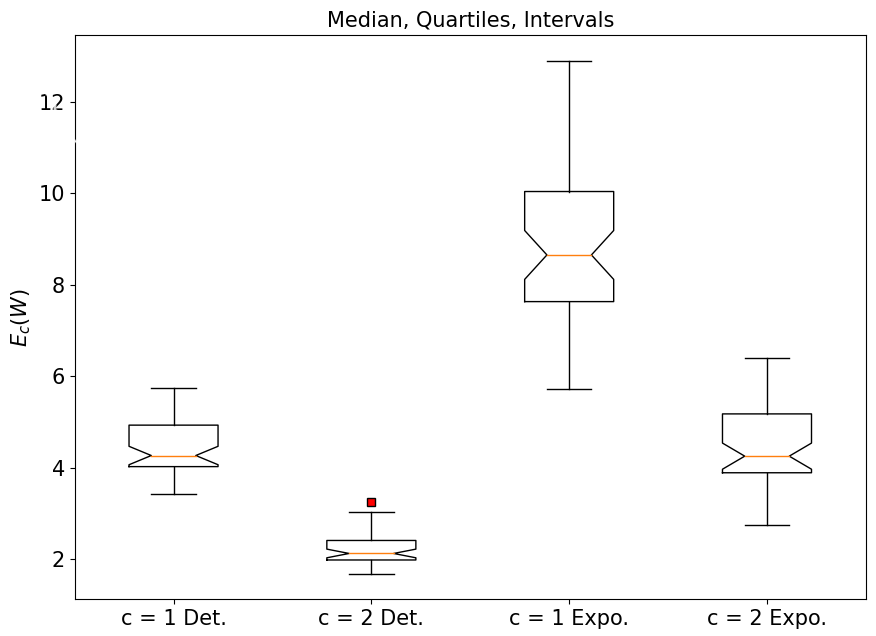
\includegraphics[width=\textwidth]{pictures/part_4/notched_box_det.png}
            \caption{Notched Box Plot, Deterministic vs  Exponential}
            \label{fig:notchedbox}
        \end{minipage}
        \hfill
        \begin{minipage}[b]{0.45\textwidth}
            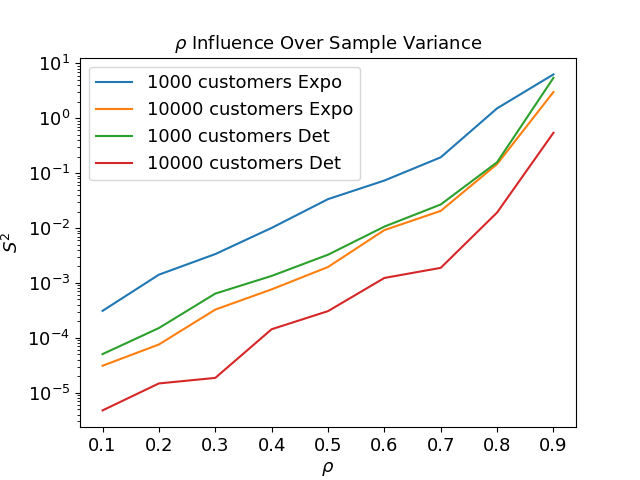
\includegraphics[width=\textwidth]{pictures/part_4/samp_var_det.png}
            \caption{Sample Variance Comparison, Semi-log Plot}
            \label{fig:samp_var_det}
        \end{minipage}
    \end{figure}

    Figure~\ref{fig:notchedbox} is a notched box plot comparing experiment results obtained using deterministic and exponential service time distributions for both $c=1$ and $c=2$. The two box plots representing the exponentially distributed wait times have significantly larger ranges, larger confidence intervals and larger medians than their deterministic counterparts. We have chosen to use the median rather than the mean because as shown earlier, our distribution doesn't tend to be completely symmetric. The deterministic service time distribution with c = 2, gives us the lowest median wait time, with a small range and tight interval, the deterministic service time distribution with c = 1 and the exponential distribution with c = 2 have similar median, but again the range and the confidence interval of the deterministic service time is substantially lower. This is confirming our hypothesis, when setting the service time distribution deterministically, we eliminate one source of stochasticity from our model, leaving the exponentially distributed arrival-times as the only stochastic component, thus it is not surprising that the output of our simulation, the expected wait time also behaves in a more deterministic way.

    In Figure~\ref{fig:samp_var_det}, we confirm that despite the lower variance $E_c(W)$ results from our deterministic service times, the sample variance of this estimator still shows the same relationship with $\rho$ as before, the same power relationship holds. However, for any given value of $\rho$ the deterministic model has a lower $S^2$ given some amount of customers.

    Finally, we will run some experiments with a hyper-exponential distribution, where 75\% of the jobs have an exponential distribution with an average service time of 1.0 and the remaining 25\% an exponential distribution with an average service time of 5. The hyper-exponential distribution has a probability density function of the form

    \begin{equation}
        f_X(x) = \sum_{i=1}^n f_{Y_i} (x) p_i
    \end{equation}

    Where $Y_i$ is a random variance sampled from the exponential distribution with a rate of $\lambda _ i$. $p_i$ is the probability that we will sample from the exponential distribution of the rate $\lambda _ i$. In our case $p_1 = 0.75, p_2 = 0.25, \lambda_1 = 1$ and $\lambda_2 = \frac{1}{5}$. We will perform some experiments with this service rate distribution for different numbers of customer slots.

    \begin{table}[h!]
        \centering
        \begin{tabular}{|c | c | c |}
            \hline
            C & $E_c(W)$ Mean & Sample Variance \\
            \hline\hline
            1 & 4480 & 46802 \\
            2 & 2222 & 9535 \\
            4 & 1114 & 2426 \\
            \hline
        \end{tabular}
        \caption{Simulation Results with a Hyperexponential Distribution of Service Times}
        \label{Table:hypexp}
    \end{table}

    Table~\ref{Table:hypexp} makes it clear that our long-tail distribution has significantly higher expected wait times than any of the other service time distributions. This is not an inherent feature of the hyper-exponential distribution but rather is a result of the parameter set we have used. The second component of the distribution with $\lambda = \frac{1}{5}$ leads to some jobs with very large service times, the length of these jobs, especially values on the long-tail of the distribution, dominate the size of the jobs generated from the component of the distribution with a smaller mean inter-service time. The sample variance values decrease significantly as we add more service slots. This is because extra slots can 'absorb' very large jobs. For instance, if $c = 1$ and a very large  service-time is sampled, everybody in the queue is held up by this job. However, if $c > 1$ then even if one server is occupied with a particularly large job, the other slots are still free to process the other jobs in the queue. Because the large job doesn't cause such a ripple effect through the queue, the impact on the wait time of other agents is reduced and thus variance of the mean wait time is reduced. This same reasoning holds for the decrease in variance between c = 2 and c = 3, but the variance reduction is smaller in this case. Partly because having two relatively large jobs be generated concurrently is not as common.

    \begin{figure}[h]
        \centering
        \begin{subfigure}[b]{0.45\linewidth}
            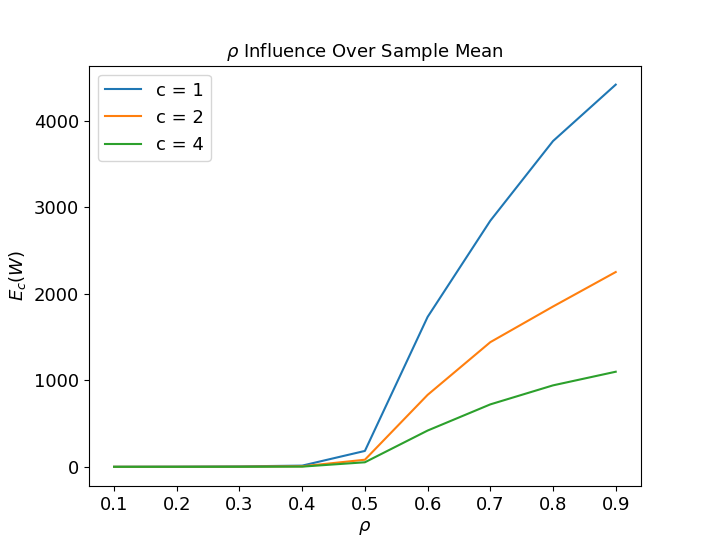
\includegraphics[width=\textwidth]{pictures/part_4/hyp_exp_mean.png}
            \vspace*{1pt}
            \caption{How the sample mean depends on $\rho$ in a hyper-exponential distribution}
            \label{fig:samp_mean_hypexp}
        \end{subfigure}
        \begin{subfigure}[b]{0.45\linewidth}
            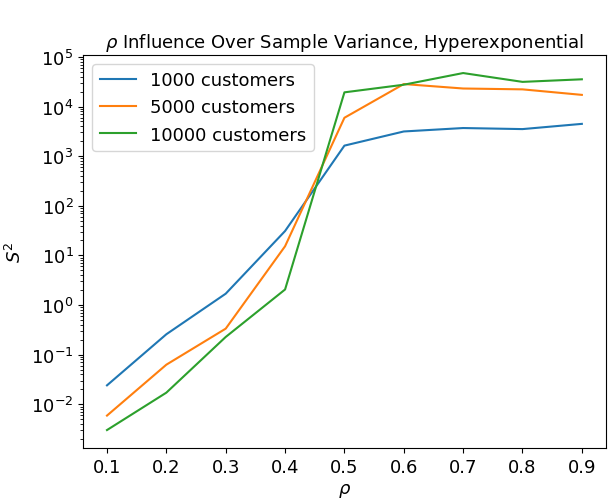
\includegraphics[width=.94\textwidth]{pictures/part_4/samp_var_hypexp.png}
            \caption{How the sample variance of our mean estimate depends on $\rho$ in a model with hyper-exponential service time distribution}
            \label{fig:samp_var_hypexp}
        \end{subfigure}
        \caption{$\rho$ influence on hyper-exponential distribution}
        \label{fig:hyperexp_sample_mean_var}
    \end{figure}

    Figure~\ref{fig:samp_mean_hypexp} shows how the sample mean for $E_c(W)$ evolves as we increase the value of $\rho$. As we would expect the wait time is increasing as we increase the system load. With a system load of less than 0.5, it makes little difference if we use more than one slot, the system is operating with some 'slack' and additional slots don't lead to any performance gain. When adding more load to the system, ($\rho > 0.5$), having access to only a single slot causes our wait time to explode, adding one or two extra slots decreases our mean wait time substantially.

    Figure~\ref{fig:samp_var_hypexp} shows the sample variance of our expected waiting time estimates for different numbers of system agents with a single slot ($c = 1$). At values of $\rho > 0.5$, the variance is quite well behaved, for a fixed value of $\rho$ a system with greater total customers has a slightly lower variance. However, when the system is overloaded ($\rho > 0.5$), more customers leads to a higher variance of our estimate. This is because at any one time, there are likely to be more agents in the queue and thus if a particularly large job is sampled from the service time distribution, then it affects a greater number of waiting customers, pushing up the expected wait time and the variance of our value.

    \section*{Conclusion}
    Throughout this paper, we have studied the queuing theory and experimented with several characteristics of well-known queue systems, such as influence of resources, service time distributions and jobs scheduling systems on the statistical properties of the expected waiting time. Our theoretical results suggested that resources (here servers) capacity would greatly influence the average waiting times, especially as the system load $\rho \rightarrow{1}$. It follows that when applying our results to a real-life system, an efficient queue should have a large margin between its actual system load and its theoretical maximal system load to maximise performance. The variance of the average waiting time will increase as well, the the waiting time becomes more unpredictable for every new jobs arriving in the queue. Our results show that for a high value of $\rho$ the distribution of average waiting time would diverge from a normal distribution if we have a large number of customers, the inverse will be true if we have a small $\rho$.

    When investigating job-first scheduling, we saw that a careful evaluation of the jobs characteristics and the choice of an adequate server disciplines  would influence as well on the efficiency of jobs sojourn time. In this specific case, as the system load $\rho$ increases above $0.5$, the usage of a non-preemptive priority discipline to schedule jobs shows obvious improvement of the median wait time in comparison to a simple first in - first out scheduling system, as well as a reduced sample variance. From our results, we come to the conclusion that an adequate queue system scheduling improves the management of jobs when the system load get closer to limits of the servers capacity.

    We then investigated the behaviour of a deterministic service time distribution, obtaining lower median wait times, a smaller range of values, tighter 95\% confidence intervals for the medians and reduced sampling variance compared to the system with exponentially distributed service times. Finally, we combined two exponential distributions with different parameters to form a hyper-exponential distribution. Broadly, we found that the component of the distribution with a smaller $\lambda$ parameter dominated the component with a larger $\lambda$ as the former component was prone to cause extremely large service times, leading to a spike in the expected wait times, especially as $\rho \rightarrow{1}$ in a $c = 1$ system.


    \clearpage

    \section*{References}

    \begin{itemize}
        \item[] Adan, Resing, 2002. Queueing Theory. Department of Mathematics and Computing Science, Eindhoven University of Technology.
        \item[] Erlang, A.K., 1920. Telephone waiting times. Matematisk Tidsskrift, B, 31, p.25.
        \item[] Kendall, D.G., 1953. Stochastic processes occurring in the theory of queues and their analysis by the method of the imbedded Markov chain. The Annals of Mathematical Statistics, pp.338-354.
        \item[] Willig, A., 1999. A short introduction to queueing theory. Technical University Berlin, Telecommunication Networks Group, 21.
    \end{itemize}

    \clearpage

\end{document}